\documentclass[reqno]{amsart}

\usepackage{amsmath, amsfonts, amssymb, hyperref,tikz}
\usepackage{graphicx}

\usetikzlibrary{matrix,arrows,shapes}
\usetikzlibrary{backgrounds}

\title{Multiplicity of P-Partition Generating Function}
\author{Tung Phan}

\newcommand{\rotate}[1]{(#1)^*}
\newcommand{\switch}[1]{\overline{(#1)}}

\newtheorem{theorem}{Theorem}
\newtheorem{corollary}{Corollary}[theorem]
\begin{document}
\maketitle

\begin{theorem} Removing/adding edges to labeled poset.\\
1. Suppose $(Q, \tau)$ is obtained from $(P, \omega)$ by deleting edges. If $(P, \omega)$ has multiplicity, so does $(Q, \tau)$.\\
2. Suppose $(P, \omega)$ is obtained from $(Q, \tau)$ by adding more edges. If $(Q, \tau)$ is multiplicity-free, so is $(P, \omega)$.
\end{theorem}
\begin{proof} \ \\
1. Let $(Q, \tau)$ inherit its labelling from $(P, \omega)$. Thus, every linear extension of $(P,\omega)$ is also a linear extension of $(Q, \tau)$. Hence, if $(P, \omega)$ has multiplicity (at least two linear extensions with the same F-function), $(Q, \tau)$ will also have such linear extensions, and thus has multiplicity. \\
2. Let $(P, \omega)$ inherit its labelling from $(Q, \tau)$. Thus, the set of linear extension of $(P, \omega)$ is a subset of the set of linear extensions of $(Q, \tau)$. If $(Q, \tau)$ is mult-free (having no two linear extensions that share the same F-function), then $(P,\omega)$ will also have no two linear extensions that share the same F-function, and thus is also mult-free.\\
\end{proof}

\begin{figure}[htbp]
\begin{center}
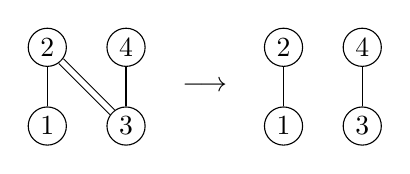
\begin{tikzpicture}[scale=1.0]
\begin{scope}
\tikzstyle{every node}=[shape=circle, inner sep=2pt]; 
\draw (0,0) node[draw] (a1) {1}; 
\draw (1,0) node[draw] (a2) {3};
\draw (0,1) node[draw] (a3) {2};
\draw (1,1) node[draw] (a4) {4};
\draw[double distance=2pt] (a2) -- (a3);
\draw (a1) -- (a3)
(a2) -- (a4); 

\begin{scope}[xshift=2cm,yshift=5mm]
\draw (0,0) node {$\longrightarrow$};
\end{scope}

\begin{scope}[xshift=3cm]
\draw (0,0) node[draw] (b1) {1}; 
\draw (1,0) node[draw] (b2) {3};
\draw (0,1) node[draw] (b3) {2};
\draw (1,1) node[draw] (b4) {4};
\draw (b1) -- (b3)
(b2) -- (b4);
\end{scope}
\end{scope}
\end{tikzpicture}
\caption{Example of deleting edges.}
\label{fig:popartitions}
\end{center}
\end{figure}

\begin{theorem} Involution \\
We consider some natural involutions we can perform on a labeled poset $(P,\omega)$. First, we can switch strict and weak edges, denoting the result $\switch{P,\omega}$. Secondly, we can rotate the labeled poset 180$^\circ$, preserving strictness and weakness of edges; we denote the resulting labeled poset $\rotate{P,\omega}$.\\

The involutions of $(P,\omega)$ will have the same multiplicity-ness as that of $(P, \omega)$. 

\end{theorem}

\begin{figure}[htbp]
\begin{center}
\begin{tikzpicture}[scale=1.0]
\matrix [row sep=20mm, column sep=20mm]  {
\node(NW) {
\begin{tikzpicture}[scale=0.8]
\tikzstyle{every node}=[draw, shape=circle, inner sep=2pt]; 
\draw (0,0) node (a1) {};
\draw (2,0) node (a2) {};
\draw (1,1) node (a3) {};
\draw (1,2) node (a4) {};
\draw (a1) -- (a3)
(a3) -- (a4);
\draw[double distance=2pt] (a2) -- (a3);
\end{tikzpicture}
};
&
\node(NE) {
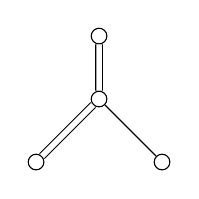
\begin{tikzpicture}[scale=0.8]
\tikzstyle{every node}=[draw, shape=circle, inner sep=2pt]; 
\draw (0,0) node (b1) {};
\draw (2,0) node (b2) {};
\draw (1,1) node (b3) {};
\draw (1,2) node (b4) {};
\draw[double distance=2pt] (b1) -- (b3)
(b3) -- (b4);
\draw (b2) -- (b3); 
\end{tikzpicture}
};
\\
\node(SW) {
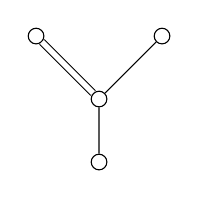
\begin{tikzpicture}[scale=0.8]
\tikzstyle{every node}=[draw, shape=circle, inner sep=2pt]; 
\draw (1,0) node (c1) {};
\draw (1,1) node (c2) {};
\draw (0,2) node (c3) {};
\draw (2,2) node (c4) {};
\draw (c1) -- (c2)
(c2) -- (c4);
\draw[double distance=2pt](c2) -- (c3);
\end{tikzpicture}
};
&
\node(SE) {
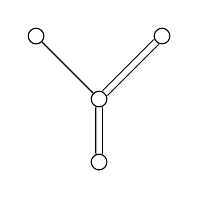
\begin{tikzpicture}[scale=0.8]
\tikzstyle{every node}=[draw, shape=circle, inner sep=2pt]; 
\draw (1,0) node (d1) {};
\draw (1,1) node (d2) {};
\draw (0,2) node (d3) {};
\draw (2,2) node (d4) {};
\draw (d2) -- (d3);
\draw[double distance=2pt](d1) -- (d2)
(d2) -- (d4);
\end{tikzpicture}
};
\\ }; 
\draw[<->,shorten >=2mm, shorten <= 2mm] (NW) -- (NE) node [midway,auto] {$\switch{P,\omega}$};
\draw[<->,shorten >=3mm, shorten <=3mm] (NW) -- (SW) node [midway,auto] {$\rotate{P,\omega}$};
\draw[<->,shorten >=3mm, shorten <=3mm] (NE) -- (SE) node [midway,auto] {$\rotate{P,\omega}$};
\draw[<->,shorten >=2mm, shorten <= 2mm] (SW) -- (SE) node [midway,auto] {$\switch{P,\omega}$};
\end{tikzpicture}
\caption{The bar and star involutions.}
\label{fig:involutions}
\end{center}
\end{figure}

\begin{theorem}
\textit{Incomparable Elements Rule}\\
Suppose $P$ contains $a,b$ with $a$ imcomparable to $b$ ($a \| b$).\\
In a linear extension of $P$ either $a$ comes before $b$ or $b$ comes before $a$. If $a$ comes before $b$ then we draw an edge from $a$ upto $b$ and vice versa.\\
Then the set of linear extensions of $P$ equals the (disjoint) union of these sets of linear extensions from each of these 2 cases.\\

\vspace{0.1in}
Let $A,B,C$ be posets. We write $A = B + C$ when $B$ and $C$ are the two cases generated from a pair of incomparable elements in $A$.\\
\end{theorem}

\begin{corollary}
If $A$ is mult-free, then so are $B$ and $C$.
\end{corollary}

\begin{corollary}
If $B$ or $C$ is not mult-free, then neiher is $A$.
\end{corollary}

\begin{corollary}
If $B$ and $C$ are mult-free, $A$ can be either mult-free or not mult-free.
\end{corollary}

\begin{figure}[htbp]
\begin{center}
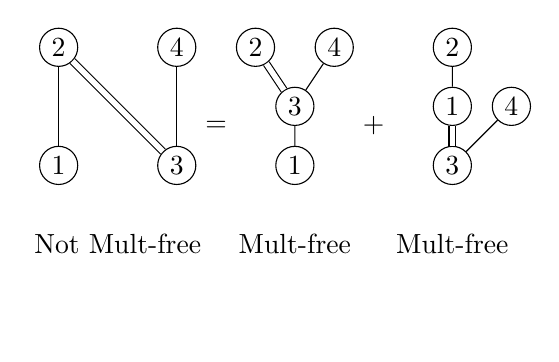
\begin{tikzpicture}[scale=1.0]
\begin{scope}
\tikzstyle{every node}=[shape=circle, inner sep=2pt]; 
\draw (0,0) node[draw] (a1) {1}; 
\draw (1.5,0) node[draw] (a2) {3};
\draw (0,1.5) node[draw] (a3) {2};
\draw (1.5,1.5) node[draw] (a4) {4};
\draw[double distance=2pt] (a2) -- (a3);
\draw (a1) -- (a3)
(a2) -- (a4); 

\begin{scope}[xshift=0.75cm,yshift=-1cm]
\draw (0,0) node {\text{Not Mult-free}};
\end{scope}

\begin{scope}[xshift=2cm,yshift=5mm]
\draw (0,0) node {=};
\end{scope}

\begin{scope}[xshift=3cm]
\draw (0,0) node[draw] (b1) {1}; 
\draw (0,0.75) node[draw] (b2) {3};
\draw (-0.5,1.5) node[draw] (b3) {2};
\draw (0.5,1.5) node[draw] (b4) {4};
\draw[double distance=2pt] (b2) -- (b3);
\draw (b1) -- (b2)
(b2) -- (b4);
\end{scope}

\begin{scope}[xshift=3cm,yshift=-1cm]
\draw (0,0) node {\text{Mult-free}};
\end{scope}

\begin{scope}[xshift=4cm,yshift=5mm]
\draw (0,0) node {+};
\end{scope}

\begin{scope}[xshift=5cm]
\draw (0,0) node[draw] (c1) {3}; 
\draw (0.75,0.75) node[draw] (c2) {4};
\draw (0,0.75) node[draw] (c3) {1};
\draw (0,1.5) node[draw] (c4) {2};
\draw[double distance=2pt] (c1) -- (c3);
\draw (c1) -- (c2)
(c3) -- (c4);
\end{scope}

\begin{scope}[xshift=5cm,yshift=-1cm]
\draw (0,0) node {\text{Mult-free}};
\end{scope}

\end{scope}
\end{tikzpicture}
\caption{Example of incomparable elements rule.}
\label{fig:popartitions}
\end{center}
\end{figure}

\begin{theorem}
(On page I1) Consider $(P,\omega)$. Suppose $P$ has maximal element $p$ such that $\omega(p)$ satisfies either\\
(i)  $\omega(p) < \omega(q)$ for all maximal elements of $(P-p,\omega)$\\
(ii) $\omega(p) > \omega(q)$ for all maximal elements of $(P-p,\omega)$\\
\vspace{5 mm}
Then $(P,\omega)$ has multiplicity if $(P-p,\omega)$ does.\\
\end{theorem}

\begin{theorem}
(Extending Theorem from I1, using idea of Bessenrodt and Willigenburg)\\
If $(P-p, \omega)$ has multiplicity, so does $(P,\omega)$ with any other elements added, as long as none of these elements are below some elements of $P$.
\end{theorem}

Implication: As long as there exist 2 linear extensions that have the same F-function and have "common" last element (vice versa, first element). We can stick any other elements to it and we will always have a not mult-free poset.

\begin{theorem} \textbf{False Theorem}\\
Supposee $(P,\omega)$ contains $(Q,\tau)$ as a convex subposet. If $(Q,\tau)$ has multiplicity, then so does $(P,\omega)$.
\end{theorem}
Implication of theorem: \textbf{False}\\
If poset $P$ contains a 3-element antichain, then $P$ has multiplicity.\\
\vspace*{5 mm}
Counter-example:

\begin{figure}[htbp]
\begin{center}
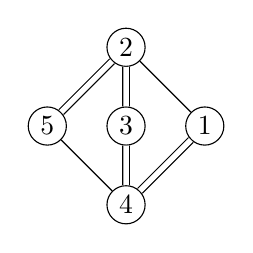
\begin{tikzpicture}[scale=1.0]
\begin{scope}
\tikzstyle{every node}=[shape=circle, inner sep=2pt]; 
\draw (0,0) node[draw] (a1) {4}; 
\draw (-1,1) node[draw] (a2) {5};
\draw (0,1) node[draw] (a3) {3};
\draw (1,1) node[draw] (a4) {1};
\draw (0,2) node[draw] (a5) {2};
\draw[double distance=2pt] (a1) -- (a3)
(a1) -- (a4)
(a3) -- (a5)
(a2) -- (a5);
\draw (a1) -- (a2)
(a5) -- (a4); 

\end{scope}
\end{tikzpicture}
\caption{Mult-free labeled poset with a 3-element antichain.}
\label{fig:popartitions}
\end{center}
\end{figure}

\end{document}
